\documentclass[12pt, titlepage]{report}
\usepackage{consumer_resource_final}
\graphicspath{{./figures/Results/feasibility}}

\begin{document}
As explained in Methods \ref{sec: methods feasibility}, before addressing the question of the stability of a system, be it dynamical or structural, it is important to study whether that system is \important{feasible}. In short we must answer the question: ``does it make sense to talk about this system? Does it even exist?''.

We will say that it makes sense to talk about a system if it is \important{feasible} (see Methods \ref{sec: methods feasibility basic concepts}). In order to be feasible, a system should respect two conditions: it must conserve biomass and its parameters must have a direct biological interpretation.

\subsection{The feasibility volume $\mathcal{V}^{G,A}_x$}
Formally we can define $\forall x \in [0,1]$ the $x$-feasibility volume $\mathcal{V}^{G,A}_x \subset \mathcal{M}$ of the consumption network coupled with the syntrophy network $(G, A) \in \mathcal{B}_{N_S \times N_R} \times  \mathcal{B}_{N_R \times N_S}$ (see Methods \ref{sec: methods feasibility volume}). Every metaparameter set $m \in \mathcal{M}$ contained in the $x$-feasibility volume $\mathcal{V}^{G,A}_x$ will give rise to a percentage $x$ of feasible systems. A first order approximation of the fully feasible volume $\mathcal{V}^{G,A}_1$ is given by Eq.\eqref{eq: fully feasible volume}.
% , which we recall here:
% \begin{equation}
% \max_i\left\{\frac{\deg(A,i)}{\deg(G,i)}\right\} \alpha_0
% \lessapprox \min(1-\sigma_0, \sigma_0) \gamma_0 R_0
% \lessapprox
% \min \left(1-\sigma_0, \sigma_0 \right) \min_\nu \left\{ \frac{l_0}{\deg(G,\nu) S_0} + \frac{\deg(A,\nu)}{\deg(G,\nu)}\alpha_0\right\}.
% \end{equation}
In the absence of syntrophy $\alpha_0=0$, it becomes:
\begin{equation}
\gamma_0 R_0 \lessapprox \frac{l_0}{\max_\nu\{\deg(G,\nu)\}S_0}. \label{eq: fully feasible volume no syntrophy}
\end{equation}
This relation is interesting in many ways. First of all it tells us that at fixed consumption rate $\gamma_0$ and resource equilibrium abundance $R_0$, feasibility increases when:
\begin{itemize}
\item the external resource input rate increases. This result was somewhat expected: if you give more food to a goldfish you expect it to thrive more.
\item the consumer equilibrium abundance $S_0$ increases. What this means is that if you want to maintain the same consumption interaction but get a higher abundance of resources at equilibrium, you must at the same time decrease the consumers equilibrium abundance.
\item the largest column-degree of the consumption matrix decreases. The degree of a given column $\nu$ of the consumption matrix tells you how many species eat from resource $\nu$. This encourages communities of specialists, where each consumer eats from its own and no other resource.
\end{itemize}
Overall we see that feasibility increases when the \important{consumption flow} $\simeq \gamma_0 S_0 \deg(G,\nu) $ is low $\forall \nu$.
Eq.\eqref{eq: fully feasible volume no syntrophy} can be confronted to simulations. First of all note that for all the matrices in the set we chose, there existed a fully feasible zone. Fortunately, there was an overlap between all of these, such that the critical feasibility $f^*(S)=1$ and the critical volume is the fully feasible volume which we denote $\mathcal{V}^1$.

 Figure \ref{fig: typical feasibility region} shows the proportion of feasible systems without syntrophy $\mathcal{F}(\gamma_0, S_0, \alpha_0=0, G)$ and $R_0=l_0=1$, $\sigma_0=0.25$ (see Methods \ref{sec: methods feasibility volume}), for two matrices $G_1$ and $G_2$ of our set. $G_1$ has connectance $\kappa_1=0.17$ and nestedness $\eta_1=0.2$, $G_2$ is more connected and more nested: $\kappa_2=0.37$ and $\eta_2=0.4$.

We observe a very sharp transition from a fully feasible to a fully unfeasible regime. Theoretically, this sharp transition happens when both sides of the inequality \eqref{eq: fully feasible volume no syntrophy} are equal, \ie at $\gamma_0 R_0 = l_0/\max_\nu\{\deg(G,\nu)\}S_0$.
 Numerically we fit the points which are at ``the boundary'' of the common feasible volume, \ie points where $0.4 \leq \mathcal{F}(\gamma_0, S_0, G) \leq 0.6$.

 For $G_1$, the theoretical expectation is $S_0 = 0.125/ \gamma_0$ and a fit on the numerical results gives $S_0=(\num[scientific-notation=false]{0.124}\pm\num{7e-8})/ \gamma_0 - (\num{6.8e-4}\pm\num{3e-7})$ so the theoretical relation is already very good.
For $G_2$, we expect $S_0 = 0.077 /\gamma_0$. A fit gives $S_0=(\num[scientific-notation=false]{0.075}\pm\num{2e-8})/\gamma_0 +(\num{3.6e-4}\pm\num{1e-7})$. Again, the theoretical value is very close to the measured value.


The numerical estimate does not always match that well the theoretical value. Fig.\ref{fig: deviation away from theory feasibility} shows the relative error $\Delta_G = 1 -$ (theoretical value)/(numerical estimate). We see that in general the theoretical expectation tends to overestimate the fully feasible region. This is probably due to the noise (\ie the deviations away from the metaparameters) in the actual systems and the structure of the $G$ matrix. Indeed Fig.\ref{fig: deviation away from theory feasibility} shows that the lower the nestedness and connectance of $G$, the worse the theoretical estimate. In the future a better approximation can surely be found taking into account the variance of the metaparameters and the nestedness of $G$.


We can similarly measure the common fully feasible volume $\mathcal{V^*}$, which according to Eq.\eqref{eq: fully feasible volume no syntrophy} is inversely proportional to the largest maximal row degree of the matrix set. For the set we considered, this yields in theory: $S_0 = 0.053 \gamma_0$. A fit on the points at the edge yields the critical boundary $S_0 = (0.043 \pm 10^{-8})/\gamma_0 - (4.6 \times 10^{-3} \pm 3 \times 10^{-8})$. The theoretical prediction is not as good as before with an error of $\sim 20 \%$. The discrepancy is probably due to the fact that numerically we determine the common feasibility volume by counting the points for which $\mathcal{F}(\gamma_0, S_0, G)=1 \ \forall G \in S_G$.
while the theoretical value matches better a fit of the points $0.4 \leq \mathcal{F} \leq 0.6$ \textbf{make this more understandable}.


\subsection{Evolution of the feasible volume with syntrophy}

Above we computed feasibles volumes when there is no syntrophy \ie $\mathcal{V}^{G}_1(\alpha_0=0)$. Since $\alpha_0=0$, we did not need to specify what the structure of $A$ was. The next naturally arising question is then: what happens to the feasible volume of a given matrix $G$ when we add a syntrophic interaction? More precisely, how does $\mathcal{V}^G_1$'s shape change?

The problem gets a bit more complex here. When we computed $\mathcal{V}^G_1(\alpha_0=0)$, we only had to take into account the structure of $G$, since there was no syntrophy. Now, we have an additional complexity because we have to think about the structure of the syntrophy network $A$ as well. The choice of $A$, which is at the core of the problem, is far from trivial. We investigated three different cases:
\begin{itemize}
  \item ``fully connected'': $A$ is filled with ones only, $A_{\mu i}=1$. This corresponds to a so-called ``mean-field'' approximation. Every consumer releases every resource at (up to some noise) the same intensity.
  \item ``no intraspecific syntrophy'': the structure of $A$ is such that consumers are not allowed to release what they consume, \ie there is no coprophagy.
  \item ``optimal LRI'': $A$ is the outcome of the Monte Carlo algorithm \footnote{Note that we took a constant value $\alpha_0$ (given in Methods \ref{section: methods LRI MC solver}) and $\gamma_0=0.2$. A more thorough analysis should build the optimal LRI matrix \important{corresponding to each $(\gamma_0, \alpha_0)$}. That would take too much time which is why we decided to keep $\gamma_0$ and $\alpha_0$ constant.}
 described in Methods \ref{section: methods LRI MC solver}, whose purpose is to make systems ``more dynamically stable'' and hence more feasible.
  \end{itemize}
  The maximal common feasible syntrophy can be estimated with the help of Eq.\eqref{eq: fully feasible volume}:
  \begin{equation}
  \alpha_0 \lessapprox \frac{\min(1-\sigma_0, \sigma_0)\gamma_0 R_0}{\max_{(G,A)\in S}\left\{\max_i\left\{\frac{\deg(A,i)}{\deg(G,i)}\right\}\right\}} \approx 0.01 \gamma_0 \leq 0.01. \label{eq : results feasibility largest alpha0}
  \end{equation}
  So we will look at ten different $\alpha_0$ values from $0$ to $0.015$. We first consider the effect of syntrophy on each consumption network $G$ then on the common fully feasible volume.

  \subsubsection{The influence of matrix structure}
  Because Eq.\eqref{eq: fully feasible volume} depends on the structure of $G$ and of $A$, we expect $\mathcal{F}^{G,A}_1$ to depend heavily on the topology of both consumption and syntrophy matrices. Figure \ref{fig: feasibility results fully feasible volume different consumption matrices} shows that indeed $\mathcal{F}^G_1$ not only changes with syntrophy but also with the network structure of the consumption matrix.

  First of all, we observe a general trend among all matrices, the fully feasible region moves horizontally to the right towards a higher $\gamma_0$. This can be explained with Eq.\eqref{eq: fully feasible volume}: when $\alpha_0 > 0$, it provides a lower bound to $\gamma_0$. Note that $S_0$ remains unbounded, so at a fixed $\gamma_0$, every $S_0$ from $0$ to the upper boundary critical curve $\sim \gamma_0^{-1}$ discussed before will be a fully feasible point. So in general, as syntrophy increases, systems with a high consumption rate and a low consumers abundance at equilibrium will remain feasible.

  Not only does $\mathcal{F}^{G,A}_1$ change its location, it also shrinks in size: as syntrophy is increased, the set of possible consumption rate and average consumers abundance is more restricted. Figure \ref{fig: feasibility results typical shrinkage of feasible volume} shows that $\text{Vol}\left(\mathcal{F}_1^G(\alpha_0)\right)$ decays exponentially as $\alpha_0$ increases.
We can define the \define{feasibility decay rate} by performing a fit in order to find the constants $c_1,c_2, d_F \in \mathbb{R}^+$ that satisfy best:
  \begin{equation}
\text{Vol}\left(\mathcal{F}_1^{G,A}(\alpha_0)\right) \approx c_1 \exp{\left(-d_F x\right)} - c_2. \label{eq: feasibility results fit feasible volume}
  \end{equation}
  The value of $d_F(G,A)$ tells us how fast the feasible volume shrinks for a given consumption-syntrophy couple $(G,A)$. In that sense $d_F(G,A)$ provides a measure of how good a consumption-syntrophy network $(G,A)$ can sustain an increase in syntrophy\footnote{One could also desire to define a \define{critical feasible syntrophy} as the smallest syntrophy that gives a zero fully feasible volume. This would be a very interesting quantity to study and could be easily found as the root of the RHS of Eq.\eqref{eq: feasibility results fit feasible volume}. We tried doing this, because the errors on $d_F$ and on the two other fitting coefficients are already quite large (see the caption of Fig.\ref{fig: feasibility results feasibility decay rate vs matrix structure}), the errors on the critical feasible syntrophy we obtained were way too large, making our results essentially meaningless.}. If $d_F$ is low then the system can bear an increase of syntrophy and stay feasible. If $d_F$ is high, the system will quickly not be feasible at all anymore.

  Figure \ref{fig: feasibility results feasibility decay rate vs matrix structure} shows how $d_F$ changes for different matrices and different structures of the syntrophy matrix. A few comments can be made. First of all it seems like the structure of $A$ does not provide any real difference, except for $G$ with $\eta_G=0.15$ and $\kappa_G=0.18$. For that specific matrix, the optimal LRI structure for $A$ reduced by a factor of three the decay rate, compared to the fully connected case. That result is only true for this specific matrix and does not hold for the others, where $d_F(G,A)$ seems to almost not depend on $A$. Furthermore a very strong trend can be observed, for all matrices and all structures of $A$: for a given connectance, $d_F$ is increased if the ecological overlap is increased and for a given ecological overlap $d_F$ decreases if the connectance is increased.
  This means clearly that systems where there is a small ecological overlap but a lot of links in the food consumption network will be favoured. Microbial communities where consumers eat from a lot of different resources (\ie each their own) can sustain a larger syntrophic interaction than others.

  %Such a fit also allows to find the \define{critical feasible syntrophy $\alpha_0^F(G,A)$}, which we define as the smallest syntrophy for which the fully feasible volume is zero. Indeed, one finds $\alpha_0^F$ by looking at the intercept of Eq.\eqref{eq: feasibility results fit feasible volume} with the $x$-axis:
  % \begin{equation}
  % \alpha_0^F(G,A) \defined -\frac{1}{c_2} \ln\left({\frac{c_3}{c_1}}\right).
  % \end{equation}

  \subsubsection{Common fully feasible volume}
 After studying the structure of each matrix individually, we can focus on the common fully feasible volume $\mathcal{F}_1^{S_M}$. Figure \ref{fig: results feasibility cfv variation with syntrophy} show the evolution of the common feasible volume as syntrophy increases. Once again, the structure of the syntrophy matrix does not seem to play a significant role in the shape of $\mathcal{F}_1^{S_M}$. Note that at $\alpha_0=\num{9.1e-3}$, $\text{Vol}\left(\mathcal{F}_1^{S_M}\right)=0$ but at $\alpha_0=\num{7.8e-3}$ the common feasible region was still non-zero. So the \define{critical common feasibility} $\alpha_0^F$, defined as the smallest syntrophy which gives rise to a zero fully feasible volume respects $\num{7.8e-3} < \alpha_0^F \leq \num{9.1e-3}$. It was estimated above that $\alpha_0^F \approx 0.01$, which is the right order of magnitude.

Figure \ref{fig: feasibility results volume of cfr depending on syntrophy} shows that unsurpisingly $\text{Vol}\left(\mathcal{F}_1^{S_M}(\alpha_0)\right)$ also decays exponentially with a rate $d_F(S_M)=\num[scientific-notation=false]{480(50)}$ per unit of syntrophy which is a bit larger than the largest $d_F(G,A)$ observed in Fig.\ref{fig: feasibility results feasibility decay rate vs matrix structure}. Without any surprise as well we observe the same shift of $\mathcal{F}_1^{S_M}$ towards points with a high $\gamma_0$ and consequently a small $S_0$ \textbf{Add interpretation on this?}.



\subsubsection{The influence of the matrix dimensions}
For now we only focused on systems with the same number of consumers and resources: $N_R=N_S=25$. But such a system lies at what has been called in the literature as May's stability bound \cite{biroli_marginally_2018}, which is precisely defined as an ecological community where the number of resources is equal to the number of species. According to the competitive exclusion principle\footnote{The heavily debated and often misunderstood \cite{hardin_competitive_1960} \important{competitive exclusion principle}, also known as Gause's principle, states that ``Complete competitors cannot coexist'' \cite{hardin_competitive_1960}, or more generally that ``the number of consumer species in steady coexistence cannot exceed that of resources'' \cite{wang_overcome_2019}.}, an ecological system which has as many resources as consumers is the border case where coexistence, \ie feasibility of our system, starts to exist, so in a way the study conducted before can be seen as a borderline case and it can be very fruitful to investigate the behaviour of systems where the number of resources has been increased to $N_R=50$.

Figure \ref{fig: feasibility results typical feasible volumes NR=50 NS=25} is the $N_R=50$ equivalent to Figure \ref{fig: feasibility results fully feasible volume different consumption matrices}. We may observe that increasing $N_R$ has a non-trivial effect, which will be different for each consumption-syntrophy network. For instance, for $G$ with $\eta_G=0.6$ and $\kappa_G=0.32$, adding more resources increases the maximal syntrophy bearable by the system (Fig.\ref{fig: feasibility results feasibility region eta 0.6 kappa 0.3}). On the contrary, for $G$ with $\eta_G=0.15$ and $\kappa_G=0.12$, it decreases it from \num{1.4e-2} to \num{7.8e-3}.

A global trend can however be discovered by looking at the common feasibility region (Fig.\ref{fig: feasibility results common feasibility region NR=50 NS=25}). We see that, compared with the $N_R=25$ case (Fig.\ref{fig: results feasibility cfv variation with syntrophy}), an overall lesser syntrophy can be achieved. Finally Figure \ref{fig: feasibility results feasibility decay rate NR=50 NS=25} shows that indeed it is really hard to predict the effect that increasing the number of resources will have on a specific consumption-syntrophy network. Indeed $d_F$, which we use to measure how big of a syntrophy a consumption-syntrophy network $(G,A)$ can bear, does not have a clear pattern, at least not under the matrix metrics we chose to measure. It is a sign that this question needs a further and deeper investigation.
\begin{figure}[h!]
\centering
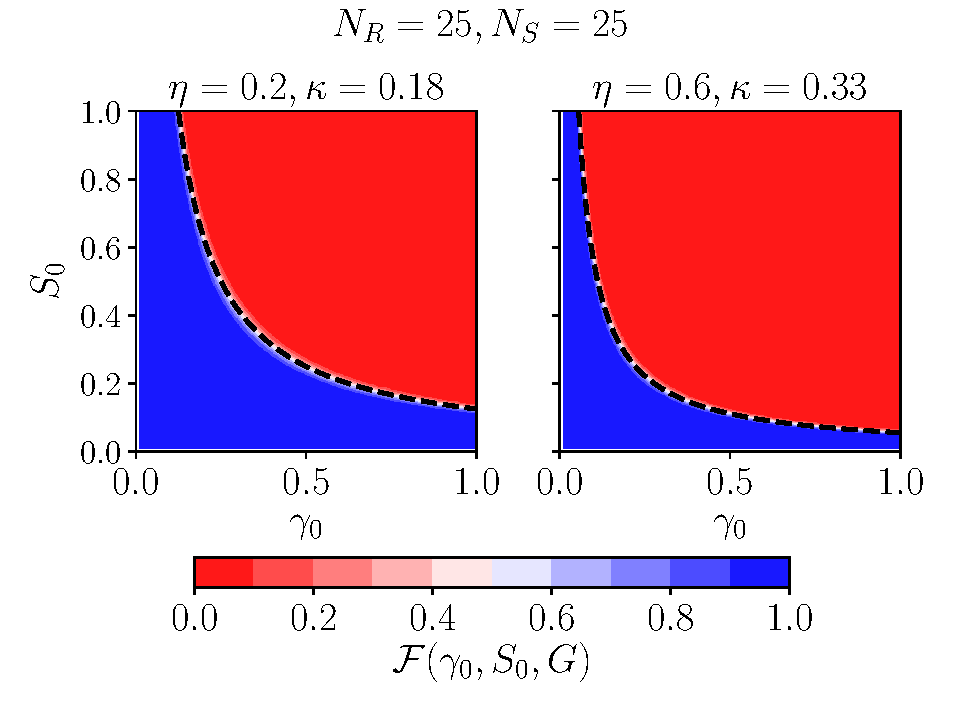
\includegraphics[width=0.7\linewidth]{typical_feasibility_volume}
\caption{Plot of the feasibility region. The color curve indicicates the feasibility function $\mathcal{F}(\gamma_0, S_0, \alpha_0=0, G)$ for $G_1$ (left) and $G_2$ (right). We observe a steep descent which marks a very clear transition from a totally feasible regime to a totally unfeasible regime, which allows us to precisely get the boundary of $\mathcal{V}^{G}_1$. The dashed lines indicate the theoretical predictions, which for both $G_1$ and $G_2$ are accurate to the order of $0.1 \%$.}
\label{fig: typical feasibility region}
\end{figure}
\begin{figure}[h!]
	\captionsetup[subfigure]{captionskip = -165pt, margin = 45pt}
\subfloat[\label{fig: deviation away from theory feasibility fixed nestedness}]{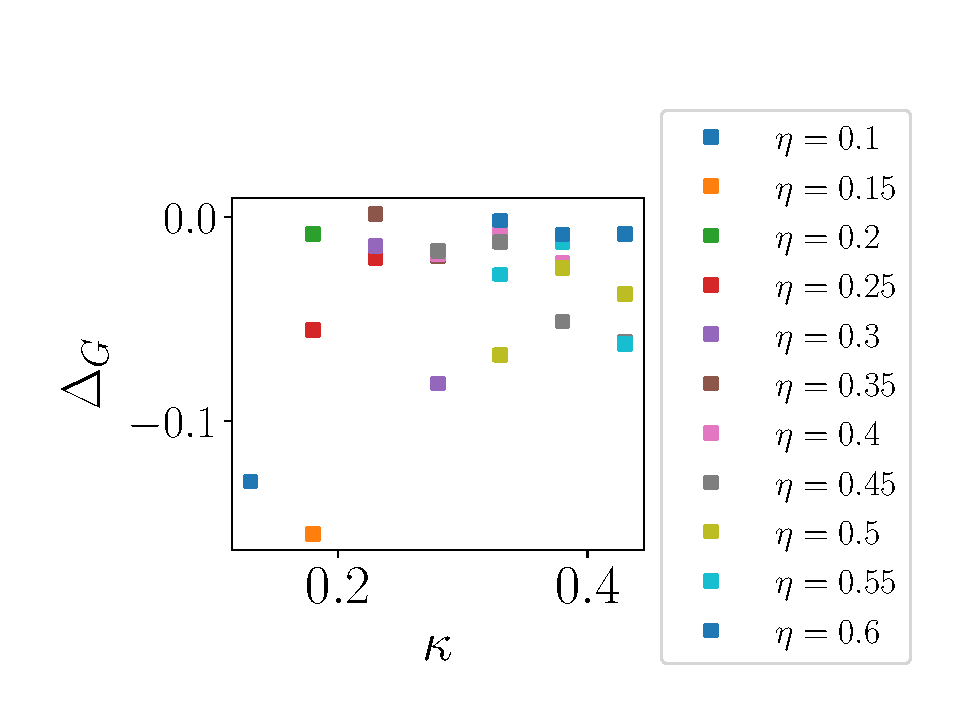
\includegraphics[width=0.49\linewidth]{feasibility_away_from_theory_fixed_nestedness}}
\captionsetup[subfigure]{captionskip = -175pt, margin = 45pt}
\subfloat[\label{fig: deviation away from theory feasibility fixed connectance}]{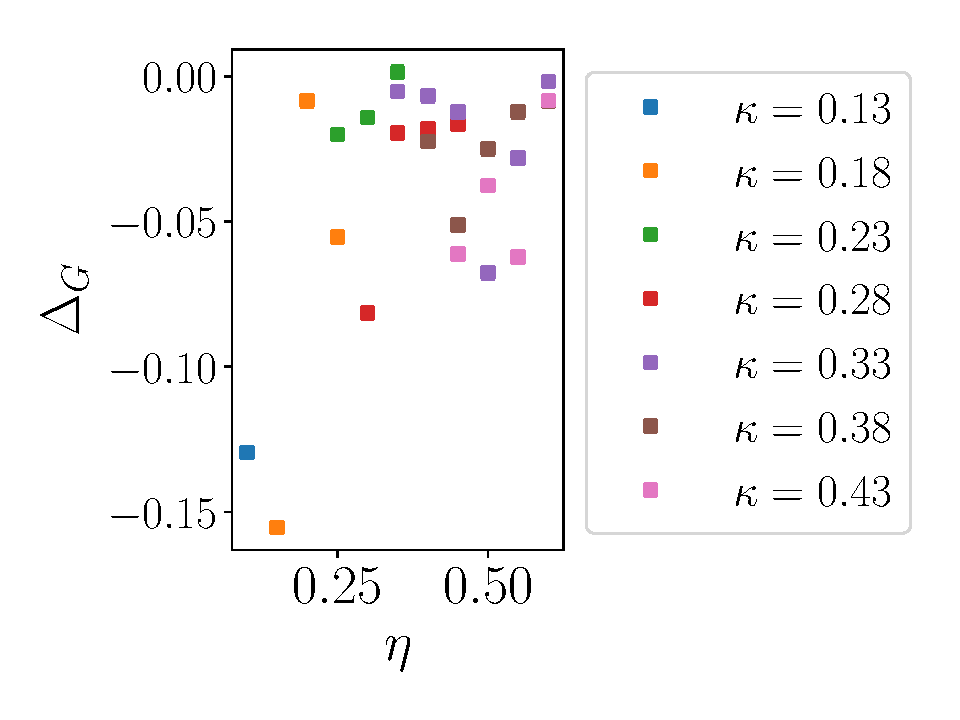
\includegraphics[width=0.49\linewidth]{feasibility_away_from_theory_fixed_connectance}}
\caption{Relative error in the determination of the boundary of $\mathcal{V}^{G,0}_1$ (a) varying connectance at fixed nestedness and (b) varying nestedness at fixed connectance. The theoretical prediction tends to overestimate the measured value. The larger the nestedness and connectance, the better the estimate.}\label{fig: deviation away from theory feasibility}
\end{figure}
\begin{figure}[h!]
\centering
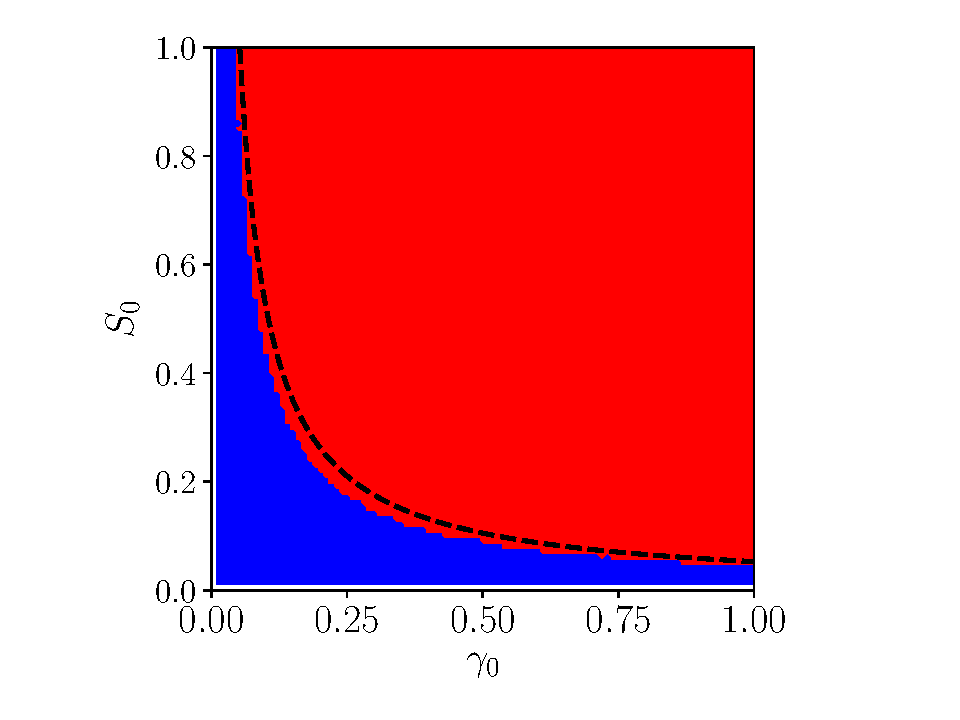
\includegraphics[width=0.7\linewidth]{common_feasibility_volume_no_syntrophy}
\caption{Plot of the common feasibility region. The blue area indicates the common feasibility volume, computed numerically, while the dashed line shows the analytical prediction. Although the match is not as good as before, the relative error is only of the order of $20 \%$. The red part is the area where not all matrices are fully feasible. From now on, it will not be considered anymore.}
\label{fig: common feasible volume}
\end{figure}
\begin{figure}
\vspace{-120pt}
\hspace{-0.1\linewidth}
\subfloat[]{\includegraphics[width=1.2\linewidth]{{feasibility_region_wt_wc_NR25_NS25_Nest0.6_Conn0.3168}.pdf}}

\vspace{-68pt}
\hspace{-0.1\linewidth}
\subfloat[]{\includegraphics[width=1.2\linewidth]{{feasibility_region_wt_wc_NR25_NS25_Nest0.35_Conn0.2208}.pdf}}

\vspace{-68pt}
\hspace{-0.1\linewidth}
\subfloat[]{\includegraphics[width=1.2\linewidth]{{feasibility_region_wt_NR25_NS25_Nest0.15_Conn0.1808}.pdf}}

\caption{Fully feasible region in the $(\gamma_0,S_0) \in [0,1] \times [0,1]$ unit square as a function of syntrophy for different consumption matrices $G$: (a)
$\eta_G=0.6$, $\kappa_G=0.32$, (b) $\eta_G=0.35$, $\kappa_G=0.22$ and (c) $\eta_G=0.15$, $\kappa_G=0.18$.
The white zone corresponds to points that are never fully feasible. The colour of a given point tells until which syntrophy that point is fully feasible, \eg
a light blue point is fully feasible for $0 \leq \alpha_0 \leq \num{9.1e-3}$. The size of the feasibility regions depend heavily on the topology of the matrix, which makes the problem far from trivial.}\label{fig: feasibility results fully feasible volume different consumption matrices}
\end{figure}
\begin{figure}
\centering
\includegraphics[width=0.6\linewidth]{{size_feasibility_region_NR25_NS25_Nest0.25_Conn0.2336}.pdf}
\caption{Decay of the volume of the fully feasible region $\mathcal{F}^G_1(\alpha_0)$ for a matrix consumption $G$ with ecological overlap $\eta_G=0.25$ and connectance $\kappa_G=0.23$ on a logarithmic scale. The solid lines represent the exponential fit explained in the main text. The three difeerent colors represent the three different structures considered for the syntrophy matrix. The decay of $\text{Vol}(\mathcal{F}^G_1)$ seems well approximated by an exponential decay and the structure of the $A$-matrix seems to not play a large role in that prospect.}
\label{fig: feasibility results typical shrinkage of feasible volume}
\end{figure}
\begin{figure}
\vspace{-84pt}
\captionsetup[subfigure]{captionskip=-190pt, margin=44pt}
\hspace{-0.1\linewidth}
\subfloat[]{\includegraphics[width=0.6\linewidth]{{feasibility_NR25_NS25_feasibility_decay_rate_fixed_nestedness_random_structure}.pdf}}
\subfloat[]{\includegraphics[width=0.6\linewidth]{{feasibility_NR25_NS25_feasibility_decay_rate_fixed_connectance_random_structure}.pdf}}

\vspace{-12pt}
\hspace{-0.1\linewidth}
\subfloat[]{\includegraphics[width=0.6\linewidth]{{feasibility_NR25_NS25_feasibility_decay_rate_fixed_nestedness_no_release_when_eat}.pdf}}
\subfloat[]{\includegraphics[width=0.6\linewidth]{{feasibility_NR25_NS25_feasibility_decay_rate_fixed_connectance_no_release_when_eat}.pdf}}

\vspace{-12pt}
\hspace{-0.1\linewidth}
\subfloat[]{\includegraphics[width=0.6\linewidth]{{feasibility_NR25_NS25_feasibility_decay_rate_fixed_nestedness_optimal_matrix}.pdf}}
\subfloat[]{\includegraphics[width=0.6\linewidth]{{feasibility_NR25_NS25_feasibility_decay_rate_fixed_connectance_optimal_matrix}.pdf}}
\caption{Feasibility decay rate for $N_R=25$ and $N_S=25$. Plots on the first column (a)-(c)-(e) show how $d_F$ changes with connectance for a given ecological overlap, while plot on the second column (b)-(d)-(f) show how it evolves when ecological overlap is changed and connectance is kept fixed. Different structures of the $A$ matrix are considered: (a)-(b) fully connected, (c)-(d) without intraspecific syntrophy and (e)-(f) outcome of the MC algorithm.}\label{fig: feasibility results feasibility decay rate vs matrix structure}
\end{figure}
\begin{figure}[h!]
\captionsetup[subfigure]{captionskip = -185pt, margin = 195pt}

\hspace{-0.1\linewidth}
\subfloat[]{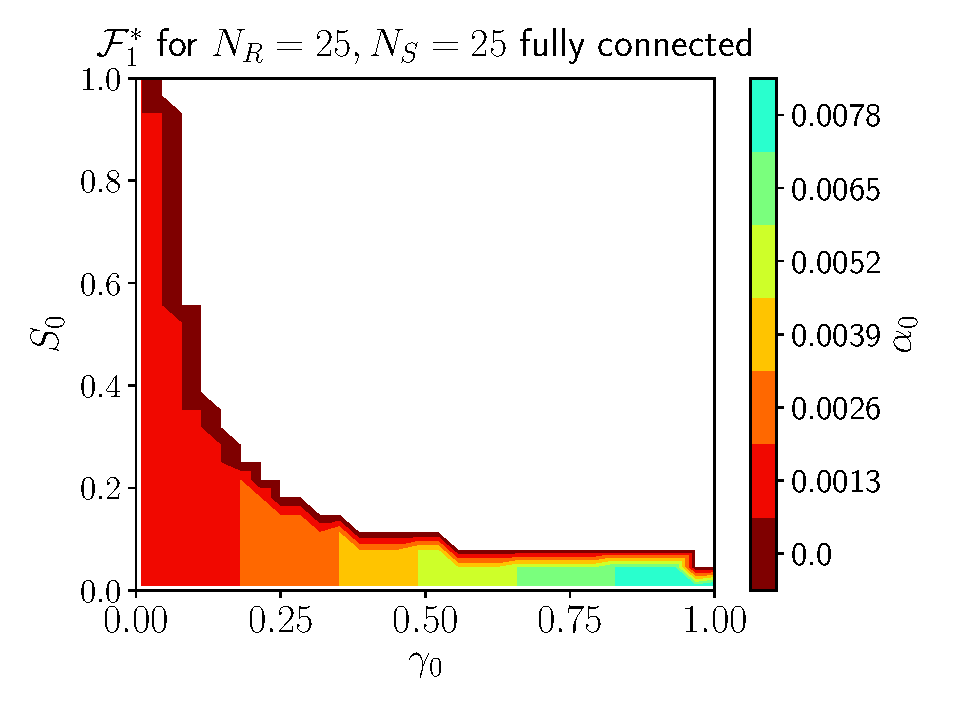
\includegraphics[width=0.6\linewidth]{common_feasibility_volume_NR25_NS25_varying_syntrophy_random_structure}}
\subfloat[]{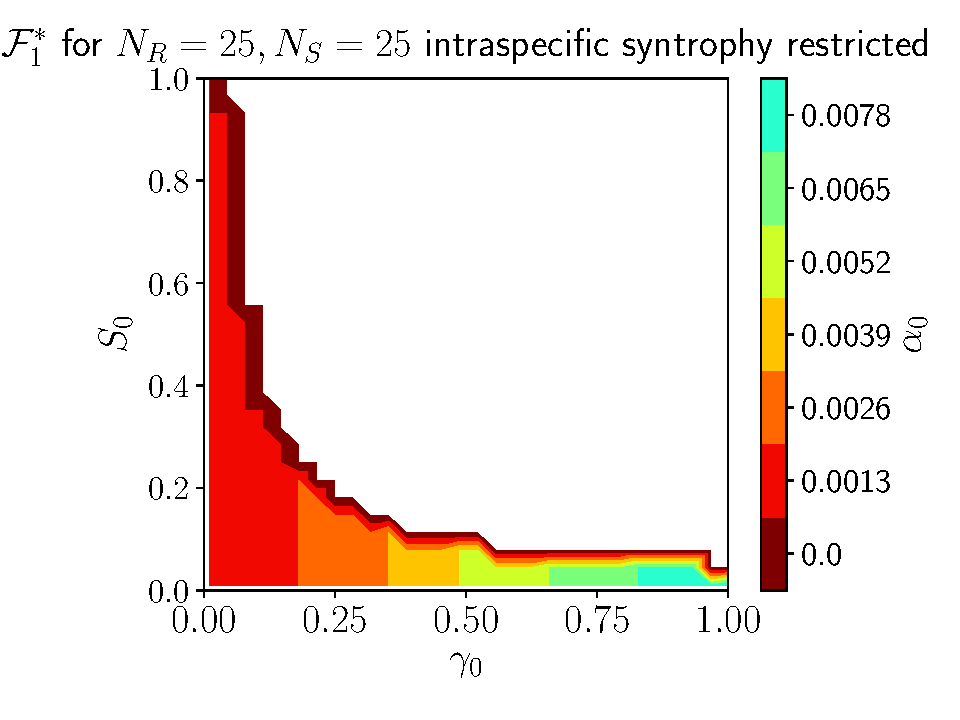
\includegraphics[width=0.6\linewidth]{common_feasibility_volume_NR25_NS25_varying_syntrophy_no_release_when_eat}}

\centering
\subfloat[]{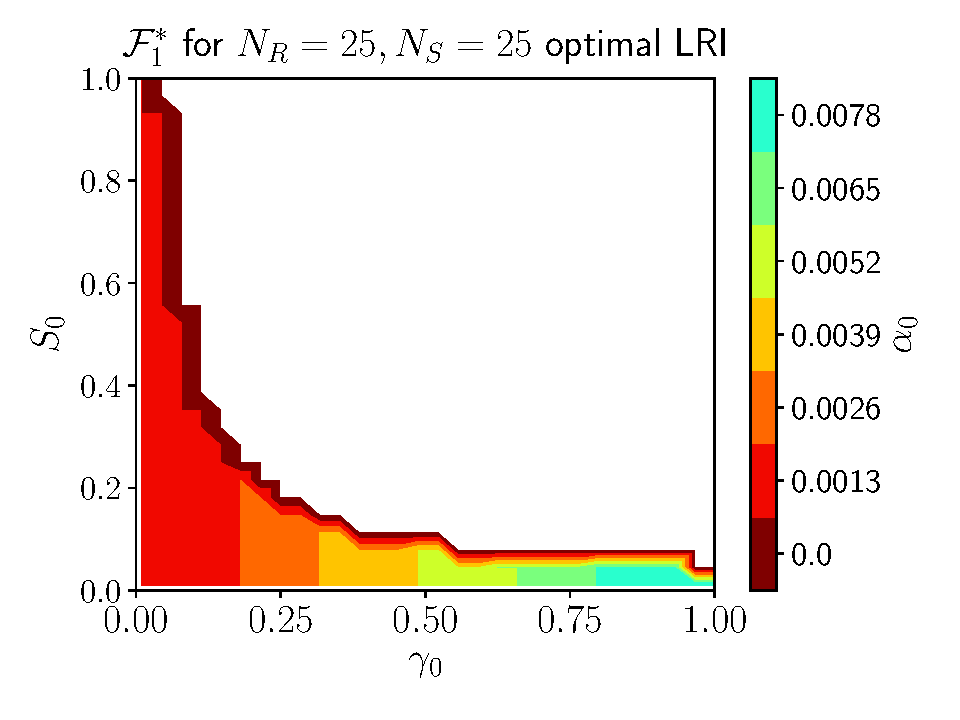
\includegraphics[width=0.6\linewidth]{common_feasibility_volume_NR25_NS25_varying_syntrophy_optimal_matrix}}

\caption[caption for LOF]{Surface plot of the fully feasible volume $\mathcal{V}^1(\alpha_0)$. The color bar on the side indicates the value of $\alpha_0$ to which the surface corresponds. The white part of the plot corresponds to points that \important{never} are fully feasible. Note that even though it is not very clear on the figure $\mathcal{V}^1(\alpha_0^+) \subset \mathcal{V}^1(\alpha_0^-) \ \forall \alpha_0^+ > \alpha_0^-$, \ie the common fully feasible region of higher syntrophy is included in the one of lower syntrophy. The different subplots correspond to different structures for the syntrophy matrix: (a) $A$ is fully connected, (b) $A$ has a structure such that intraspecific syntrophy is restricted and (c) $A$ is obtained through the LRI MC algorithm described in Methods \ref{section: methods LRI MC solver}.} \label{fig: results feasibility cfv variation with syntrophy}
\end{figure}
\begin{figure}
\centering
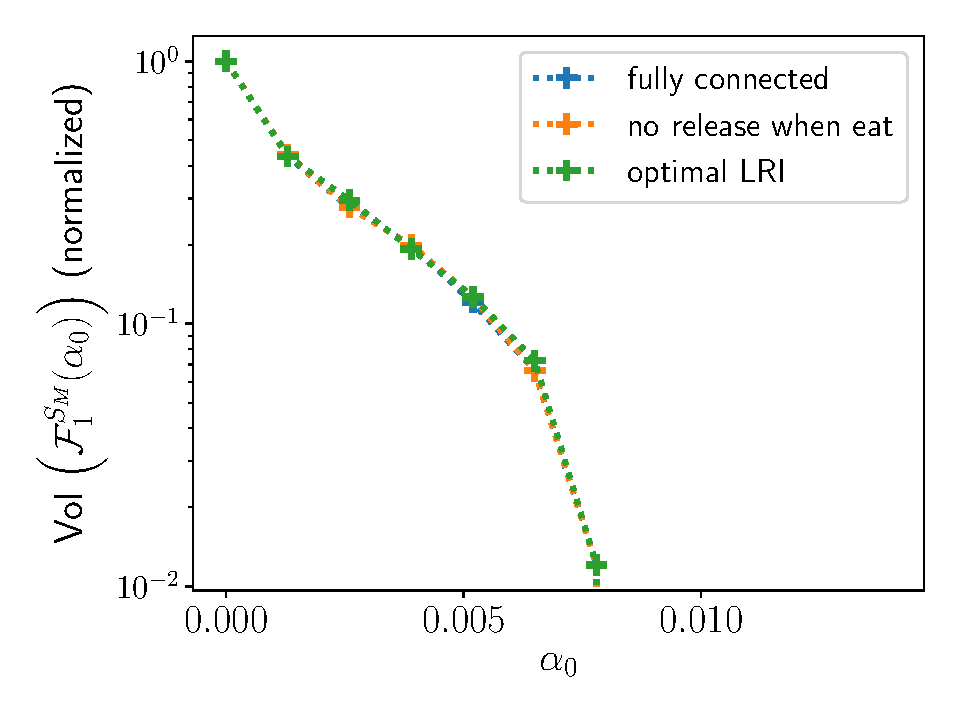
\includegraphics[width=0.7\linewidth]{measure_common_feasibility_volume_varying_syntrophy}
\caption{Volume of the common feasibility region $\mathcal{V}^1(\alpha_0)$ as a function of syntrophic interaction strength $\alpha_0$. The curves indicate the different structures used for the syntrophy network $A$.}\label{fig: feasibility results volume of cfr depending on syntrophy}
\end{figure}

\begin{figure}
\vspace{-120pt}
\hspace{-0.05\linewidth}
\subfloat[\label{fig: feasibility results feasibility region eta 0.6 kappa 0.3}]{\includegraphics[width=1.1\linewidth]{{feasibility_region_wt_NR50_NS25_Nest0.6_Conn0.3344}.pdf}}

\vspace{-28pt}
\hspace{-0.05\linewidth}
\subfloat[]{\includegraphics[width=1.1\linewidth]{{feasibility_region_wt_NR50_NS25_Nest0.35_Conn0.2296}.pdf}}

\vspace{-28pt}
\hspace{-0.05\linewidth}
\subfloat[\label{fig: feasibility results feasibility region eta 0.15 kappa 0.12}]{\includegraphics[width=1.1\linewidth]{{feasibility_region_wt_NR50_NS25_Nest0.15_Conn0.12}.pdf}}
\vspace{-12pt}
\caption{Surface colour plot of the fully feasible region $\mathcal{F}_1^{G,A}\left(\alpha_0\right)$ as a function of the syntrophy $\alpha_0$ for the case $N_R=50$, with different structures of $A$: fully connected (left column), no intraspecific syntrophy (middle) and LRI matrix (right). The rows correspond to different choices of the consumption matrix $G$: (a) $\eta_G=0.6$ and $\kappa_G=0.33$, (b) $\eta_G=0.35$ and $\kappa_G=0.23$, (c) $\eta_G=0.15$ and $\kappa_G=0.12$. These are matrices with similar properties than  Fig.\ref{fig: feasibility results fully feasible volume different consumption matrices}, except that the number of resources is here doubled. This affects $\mathcal{F}_1^{G,A}\left(\alpha_0\right)$ quite drastically.}\label{fig: feasibility results typical feasible volumes NR=50 NS=25}
\vspace{-60pt}
\end{figure}
\begin{figure}[h!]
\captionsetup[subfigure]{captionskip = -185pt, margin = 195pt}

\hspace{-0.1\linewidth}
\subfloat[]{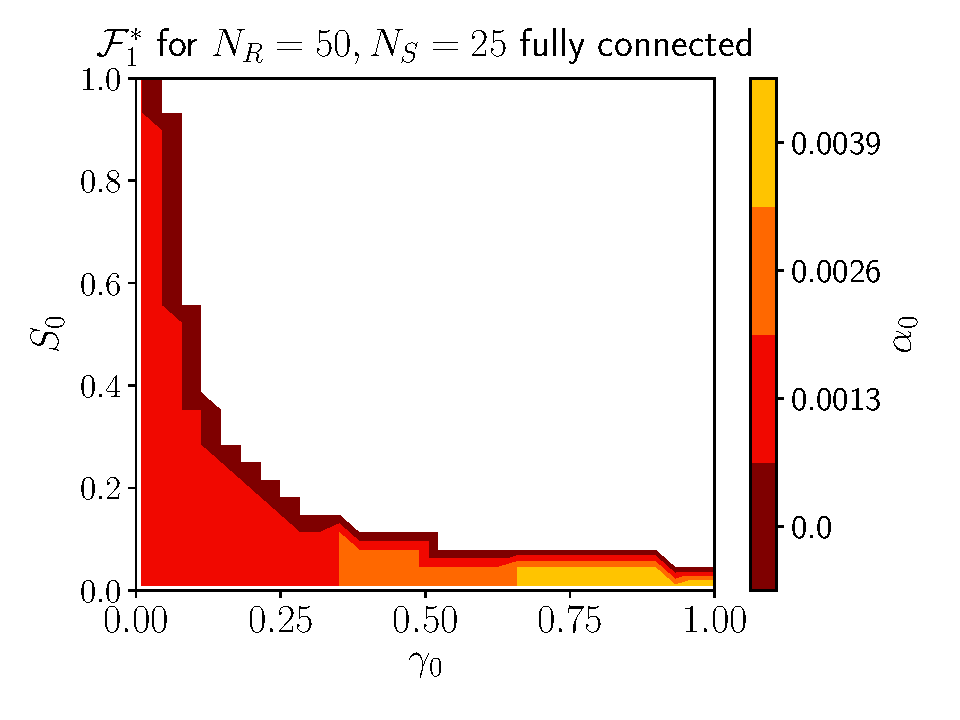
\includegraphics[width=0.6\linewidth]{common_feasibility_volume_NR50_NS25_varying_syntrophy_random_structure}}
\subfloat[]{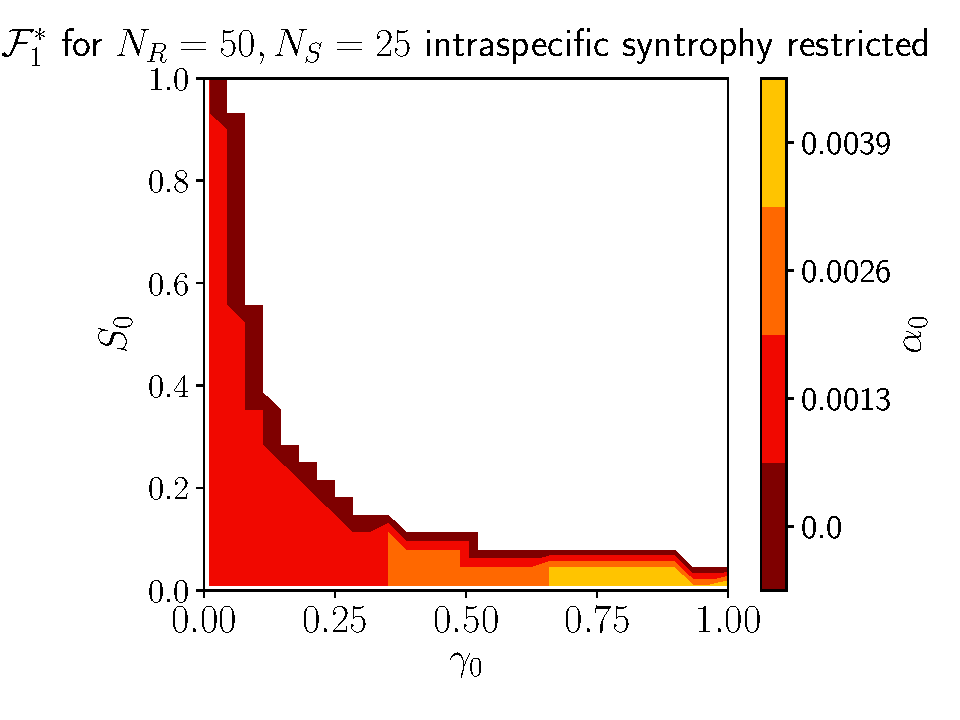
\includegraphics[width=0.6\linewidth]{common_feasibility_volume_NR50_NS25_varying_syntrophy_no_release_when_eat}}

\centering
\subfloat[]{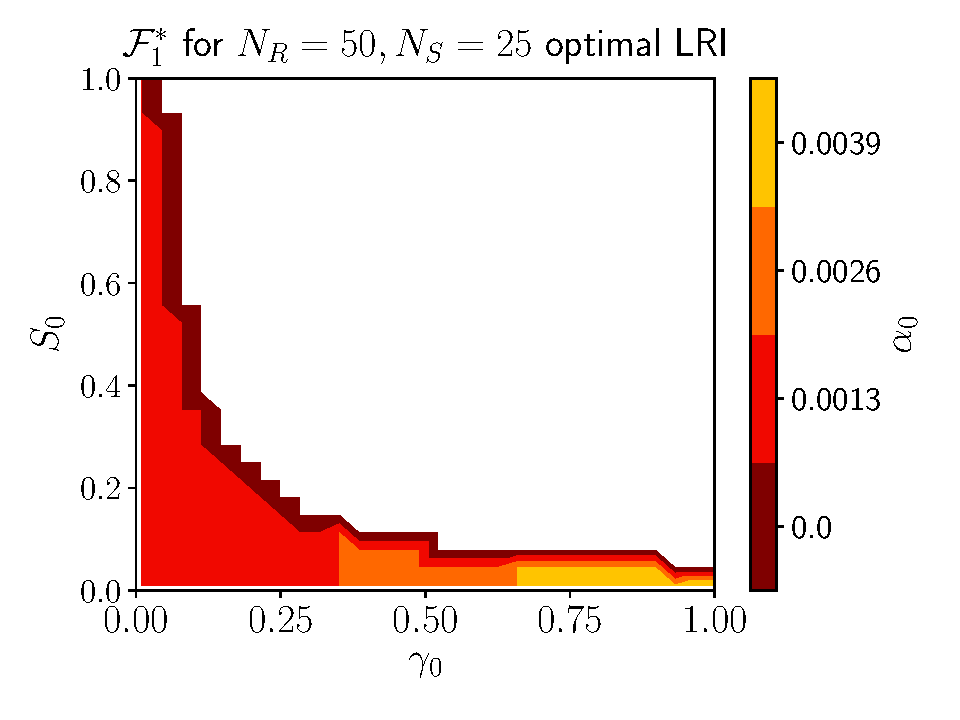
\includegraphics[width=0.6\linewidth]{common_feasibility_volume_NR50_NS25_varying_syntrophy_optimal_matrix}}
\caption{Common feasibility region $\mathcal{F}_1^{S_M}\left(\alpha_0\right)$ for $N_R=50$ and $N_S=25$, to compare with \ref{fig: results feasibility cfv variation with syntrophy}. We considered different structures of the syntrophy matrix: (a) fully connected, (b) intraspecific syntrophy restricted and (c) LRI matrix. As the number of resources increases, the feasibility volume for a given $\alpha_0$ decreases.}\label{fig: feasibility results common feasibility region NR=50 NS=25}
\end{figure}

\begin{figure}
\vspace{-84pt}
\captionsetup[subfigure]{captionskip=-190pt, margin=48pt}
\hspace{-0.1\linewidth}
\subfloat[]{\includegraphics[width=0.6\linewidth]{{decay_rate_25_vs_50_nestedness_random_structure}.pdf}}
\subfloat[]{\includegraphics[width=0.6\linewidth]{{decay_rate_25_vs_50_connectance_random_structure}.pdf}}

\vspace{-12pt}
\hspace{-0.1\linewidth}
\subfloat[]{\includegraphics[width=0.6\linewidth]{{decay_rate_25_vs_50_nestedness_no_release_when_eat}.pdf}}
\subfloat[]{\includegraphics[width=0.6\linewidth]{{decay_rate_25_vs_50_connectance_no_release_when_eat}.pdf}}

\vspace{-12pt}
\hspace{-0.1\linewidth}
\subfloat[]{\includegraphics[width=0.6\linewidth]{{decay_rate_25_vs_50_nestedness_optimal_matrix}.pdf}}
\subfloat[]{\includegraphics[width=0.6\linewidth]{{decay_rate_25_vs_50_connectance_optimal_matrix}.pdf}}
\caption{Comparison of the feasibility decay rates obtained for matrices with same ecological and connectance, at $N_R=25$ and $N_R=50$. The color of the points indicates their ecological overlap (left) or connectance (right). The straight line represents equal $d_F(N_R=50)$ and $d_F(N_R=25)$.  Different structures for the syntrophy matrix $A$ are considered: (a) fully connected, (b) no intraspecific syntrophy and (c) LRI matrix. No clear tendency on what effect increasing resources will have can be drawn.}
\label{fig: feasibility results feasibility decay rate NR=50 NS=25}
\end{figure}




\end{document}
